\documentclass[aspectratio=169,t,xcolor=table]{beamer}
\usepackage{multirow}
\usepackage[portuges]{babel}
\usepackage[utf8x]{inputenc}
\usepackage[T1]{fontenc}
\usepackage{booktabs}
\usepackage{subcaption}
\usepackage[percent]{overpic}
\usepackage{multicol}
\usepackage{soul}
\usepackage{tikz}
\usetikzlibrary{arrows.meta}
\usetikzlibrary{positioning}
\usepackage{color}
\definecolor{red}{RGB}{255,0,0}
\usepackage[makeroom]{cancel}
\renewcommand{\CancelColor}{\color{red}}
\usetheme{Ufg}

%-------------------------------------theorems--------------
\newtheorem{conj}{Conjetura}
\newtheorem{defi}{Definição}
\newtheorem{teo}{Teorema}
\newtheorem{lema}{Lema}
\newtheorem{prop}{Proposição}
\newtheorem{cor}{Corolário}
\newtheorem{ex}{Exemplo}
\newtheorem{exer}{Exercício}

\setbeamertemplate{theorems}[numbered]
\setbeamertemplate{caption}[numbered]

%-------------------------------------------------------------%
%----------------------- Primary Definitions -----------------%

% This command set the default Color, is also possible to choose a custom color (beamerthemeUfg.sty)
\setPrimaryColor{CustomBlue}

% First one is logo in title slide (we recommend use a horizontal image), and second one is the logo used in the remaining slides (we recommend use a square image)
\setLogos{lib/logos/usp.png}{lib/logos/pipges.png}{lib/logos/pipges_75.png}


% -------------------------------------- Title Slide Information
\title[Inf PIPGES]{Representer Theorem}

% \author[Discente, Docente]{Gabriel de Jesus Pereira\inst{1} \and Vera Lucia Damasceno Tomazella}
\author[Discente, Docente]{Gabriel de Jesus Pereira\inst{1} \and Vera Lucia Damasceno Tomazella}

\institute[UFSCar] % (optional)
{
  \inst{1}%
  Mestrado - PIPGEs\\
%   Doutorado - PIPGEs\\
  UFSCar \& USP \\
  %Houve financiamento?
  %\vspace{.2in} {\Large \textbf{Pesquisa financiada pela CAPES}}
}
\date{\today}

%-----------------------The next statement creates the title page.
\begin{document}
\frame[noframenumbering]{\titlepage}


%------------------------------------------------Slide 1
\setLayout{vertical} % This command define the layout. 'vertical' can be replace with 'horizontal', 'blank, 'mainpoint', 'titlepage'

\section{Nome da seção}

\setLayout{mainpoint}

\begin{frame}
% 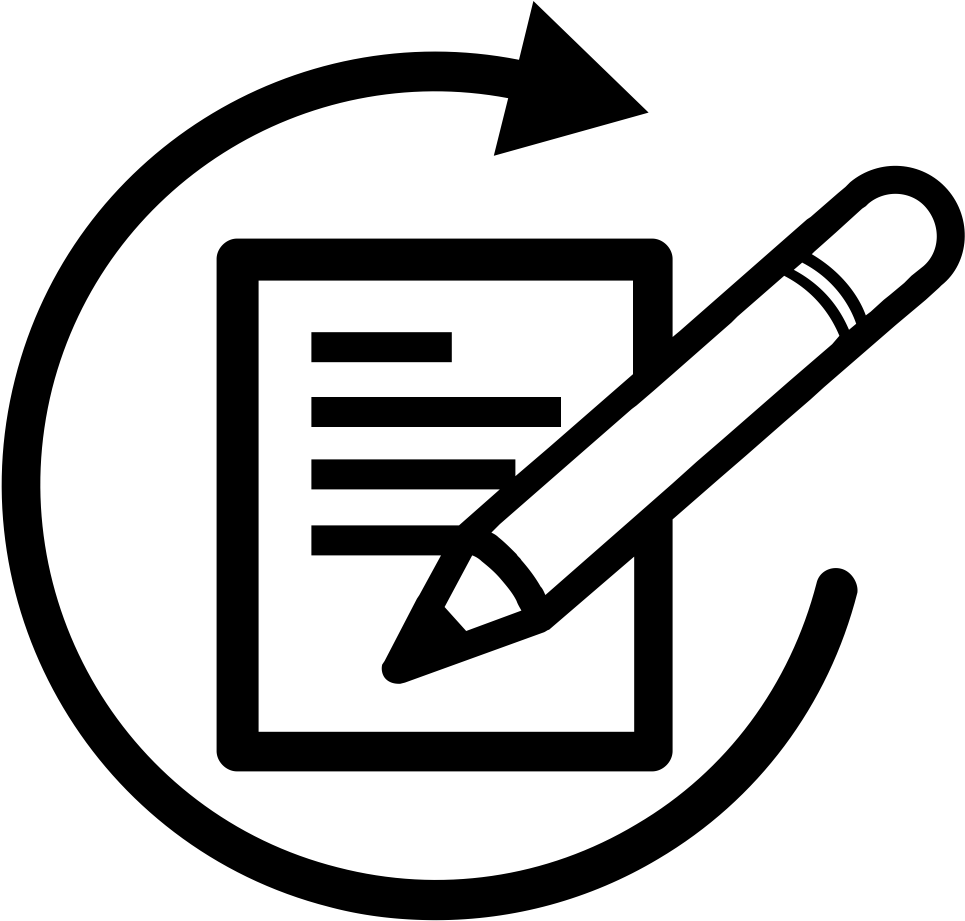
\includegraphics[width = .25\linewidth]{Images/evaluate.png} %Adiciona imagem
\frametitle{\Huge Representer Theorem}
\end{frame}

%------------------------------------------------Slide 2
\setLayout{vertical}
\begin{frame}{Por que é importante?}

\begin{itemize}
    \item Muitos problemas minimizam:

    \vfill

    \[
    \mathcal{L}(h(x_1), \dots, h(x_n)) + \lambda \|h\|_{\mathcal{H}}^2
    \]

    \vfill

    \item Mas $\mathcal{H}$ pode ser infinito-dimensional

    \vfill
    % \vspace{0.3cm}

    \item Como otimizar sobre infinitas funções?

    \vfill
    % \vspace{0.3cm}

    \item O Teorema do Representante fornece a resposta.
\end{itemize}

\end{frame}

%------------------------------------------------Slide 3
\begin{frame}{Intuição}

\begin{itemize}
    \item A perda depende apenas de:

    \vfill

    \[
    h(x_1), \dots, h(x_n)
    \]

    \vfill

    \item Portanto, apenas o comportamento no conjunto de treino importa

    \vfill

    \item Qualquer componente extra fora dessas observações apenas aumenta a complexidade

    \vfill

    \item A melhor solução pertence a um subespaço de dimensão finita
\end{itemize}

\end{frame}


\begin{frame}{Intuição}

\centering

\begin{tikzpicture}[scale=1.1]

% Eixos
\draw[->] (0,0,0) -- (5,0,0) node[right] {$x_1$};
\draw[->] (0,0,0) -- (0,4,0) node[above] {$x_2$};
\draw[->] (0,0,0) -- (0,0,4) node[left] {$x_3$};

% Plano x3 = 0
\filldraw[fill=blue!10,opacity=0.5]
(0,0,0) -- (4,0,0) -- (4,3,0) -- (0,3,0) -- cycle;

\node at (4.4,2.8,0) {$x_3=0$};

% Classe +
\filldraw[red] (1,1,0) circle (2pt);
\filldraw[red] (1.4,1.8,0) circle (2pt);
\filldraw[red] (2,1.2,0) circle (2pt);

% Classe -
\filldraw[black] (3,2.2,0) circle (2pt);
\filldraw[black] (3.3,1.3,0) circle (2pt);
\filldraw[black] (2.8,0.8,0) circle (2pt);

% Hiperplano vertical
\filldraw[fill=green!20,opacity=0.4]
(2.4,0,0) --
(2.4,3,0) --
(2.4,3,3) --
(2.4,0,3) -- cycle;

\node at (2.7,3.2,2) {$\mathbf{w}^\top x + b = 0$};

% Vetor normal no plano x1-x2
\draw[->, thick, red] (2.4,1.5,0) -- (3.3,1.5,0);
\node[above] at (3.3,1.5,0) {$\mathbf{w}$};

\end{tikzpicture}

\vspace{0.4cm}

\begin{itemize}
    \item Os dados vivem no plano \(x_3=0\)
    \item Logo, a direção \(x_3\) não influencia a separação
    \item Portanto, \(w_3 = 0\)
\end{itemize}

\end{frame}


%------------------------------------------------Slide 5
\begin{frame}{Representer theorem}

\vfill

% \begin{teo}

Seja $K\text{ : } \mathcal{X} \times \mathcal{X} \to \mathbb{R}$ um kernel PDS e $\mathcal{H}$
seu RHKS correspondente. Então, para qualquer função não-descrescente $G\text{ : } \mathbb{R} \to \mathbb{R}$
e qualquer função de perda $\mathcal{L}\text{ : } \mathbb{R}^n \to \mathbb{R} \cup \{+\infty\}$, a solução do problema

\[
\arg\min_{h\in \mathcal{H}} \left\{ \mathcal{L}(h(x_1), \dots, h(x_n)) + G(\|h\|_{\mathcal{H}}) \right\}
% {\arg\min}_{h \in \mathcal{H}} \left\{ \mathcal{L}(h(x_1), \dots, h(x_n)) + \lambda \|h\|_{\mathcal{H}}^2 \right\}
\]

% \[
% \min_{f \in \mathcal{H}}
% \left\{
% \mathcal{L}(f(x_1), \dots, f(x_n))
% +
% \lambda \|f\|_{\mathcal{H}}^2
% \right\}
% \]

admite uma solução na forma

\[
h^*(x)=\sum_{i=1}^{n}\alpha_i K(x_i,x)\text{.}
\]

% \end{teo}

\end{frame}

%------------------------------------------------Slide 6
\begin{frame}{O que isso significa?}

\begin{itemize}
    \item Problema de dimensão infinita

    % [
    % \Downarrow
    % \]
    \vfill

    \item Otimização em dimensão finita

    % \[
    % \Downarrow
    % \]
    \vfill

    \item Apenas os coeficientes $\alpha_1,\dots,\alpha_n$ são necessários

    \vfill

    \item Métodos de kernel tornam-se computacionalmente viáveis
\end{itemize}

\end{frame}

\setLayout{mainpoint}

\begin{frame}
% 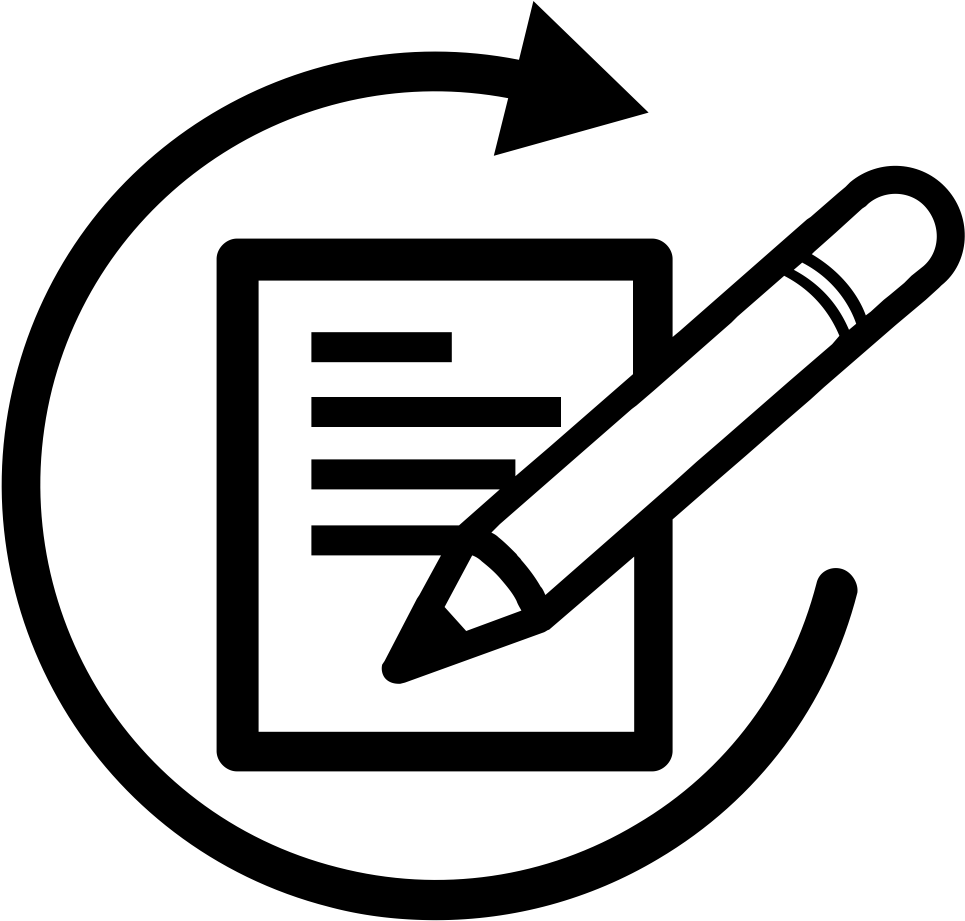
\includegraphics[width = .25\linewidth]{Images/evaluate.png} %Adiciona imagem
\frametitle{\Huge Exemplo de aplicação do Representer Theorem}
\end{frame}

%------------------------------------------------Slide 7
\setLayout{vertical}

\begin{frame}{Kernel Ridge Regression}

No Kernel Ridge Regression, resolvemos:

\[
\begin{aligned}
\min_{\mathbf{w}} \quad &
\sum_{i=1}^n
\left(
\mathbf{w}\cdot\Phi(x_i)-y_i
\right)^2
+
\lambda \|\mathbf{w}\|^2
\end{aligned}
\]

Pelo Teorema do Representante, a solução ótima deve pertencer ao subespaço gerado por:

\[
\mathbf{w}
=
\sum_{i=1}^n
\alpha_i \Phi(x_i)
\]

Substituindo essa representação no modelo:

\[
h(x)
=
\mathbf{w}\cdot\Phi(x)
=
\sum_{i=1}^n
\alpha_i K(x_i,x)
\]


\end{frame}


\begin{frame}{Support Vector Machine}

No Support Vector Machine (sem intercepto), resolvemos:

\[
\begin{aligned}
\min_{f \in \mathcal{H}} \quad &
\frac{1}{n}\sum_{i=1}^{n}\max\left(0,1-y_if(x_i)\right)
+ \frac{\lambda}{2}\|f\|_{\mathcal H}^2
\end{aligned}
\]

Pelo Teorema do Representante, a solução ótima tem a forma:

\[
f(x)=\sum_{i=1}^{n}\alpha_iK(x_i,x)
\]

Substituindo na otimização:

\[
\begin{aligned}
\min_{\alpha}\quad &
-\sum_{i=1}^{n}\alpha_i
+
\frac12\sum_{i=1}^{n}\sum_{j=1}^{n}
y_iy_j\alpha_i\alpha_jK(x_i,x_j)\quad &
\text{sujeito a}\quad &
0\leq \alpha_i \leq \frac{1}{n\lambda}
\end{aligned}
\]

\end{frame}

%------------------------------------------------Conclusão
\section{Conclusão}

\setLayout{mainpoint}

\begin{frame}
\frametitle{\Huge Conclusão}
\end{frame}

%------------------------------------------------Slide conclusão
\setLayout{vertical}

\begin{frame}{Conclusões}

\begin{itemize}
    \item O Teorema do Representante reduz problemas de dimensão infinita para dimensão finita

    \vspace{0.4cm}

    \item A solução ótima pertence ao subespaço gerado pelos dados:

    \[
    f^*(x)=\sum_{i=1}^n \alpha_i K(x_i,x)
    \]

    \vspace{0.4cm}

    \item Isso torna métodos de kernel computacionalmente viáveis

    \vspace{0.4cm}

    \item Kernel Ridge Regression e SVM são aplicações diretas desse resultado

\end{itemize}

\end{frame}

%------------------------------------------------Referências
\section{Referências}

\setLayout{mainpoint}

% \setLayout{vertical}
% \begin{frame}[allowframebreaks]{Referências}
% \bibliographystyle{plain}
% \bibliography{references}

% \cite{mohri2018foundations}
% \end{frame}

\begin{frame}
\frametitle{\Huge Referências}
\end{frame}

%------------------------------------------------Slide referências
\setLayout{vertical}

\begin{frame}[allowframebreaks]{Referências}

\footnotesize
\bibliographystyle{plain}
\bibliography{references}

\cite{mohri2018foundations}

\cite{wahba2019representer}

\end{frame}

\end{document}
